%\title{Article HW Template}

\documentclass[12pt]{article}

\usepackage{graphicx} % Required for including pictures
%\graphicspath{{Images/}} % Specifies the directory where pictures are stored
\usepackage[figurename=Figure]{caption}
\usepackage{float}    % For tables and other floats
\usepackage{verbatim} % For comments and other
\usepackage{amsmath}  % For math
\usepackage{amssymb}  % For more math
\usepackage{fullpage} % Set margins and place page numbers at bottom center
\usepackage{paralist}
\usepackage{listings} % For source code
\usepackage{subfig}   % For subfigures
\usepackage{booktabs}
%\usepackage[usenames,dvipsnames]{color} % For colors and names
%\usepackage[pdftex]{hyperref}           % For hyperlinks and indexing the PDF
%\hypersetup{ % play with the different link colors here
%    colorlinks,
%    citecolor=blue,
%    filecolor=blue,
%    linkcolor=blue,
%    urlcolor=blue % set to black to prevent printing blue links
%}

\newcommand{\boxitem}[2]{\vspace{.55cm}
	\item[#1]
	\leavevmode
	\strut
	\vadjust{%%
		\noindent
		\raisebox{\dimexpr\dp\strutbox+\ht\strutbox+1ex}[0pt][0pt]{\tikzmark{bl}}}%%
	#2
	
	\leavevmode
	\vadjust{%
		\noindent
		\hspace*{\dimexpr\textwidth+1ex}\tikzmark{br}}%%
	
	\tikz[overlay,remember picture]{\draw[black]
		(bl) rectangle
		(br);}}

\newcommand{\tikzmark}[1]{\tikz[overlay,remember picture] \node (#1) {};}

\usepackage{tikz} % To generate the plot from csv
\usetikzlibrary{shapes,arrows,positioning,calc}



\usepackage{pgfplotstable}
\usepackage{pgfplots}
\pgfplotsset{compat=1.5}

\pgfplotsset{compat=1.7}
\definecolor{mygreen}{RGB}{28,172,0} % color values Red, Green, Blue
\definecolor{mylilas}{RGB}{170,55,241}
\lstset{language=Matlab,%
	%basicstyle=\color{red},
	breaklines=true,%
	morekeywords={matlab2tikz},
	keywordstyle=\color{blue},%
	morekeywords=[2]{1}, keywordstyle=[2]{\color{black}},
	identifierstyle=\color{black},%
	stringstyle=\color{mylilas},
	commentstyle=\color{mygreen},%
	showstringspaces=false,%without this there will be a symbol in the places where there is a space
	%numbers=left,%
	%numberstyle={\tiny \color{black}},% size of the numbers
	%numbersep=9pt, % this defines how far the numbers are from the text
	emph=[1]{for,end,break},emphstyle=[1]\color{red}, %some words to emphasise
	%emph=[2]{word1,word2}, emphstyle=[2]{style},    
}

%Block Diagram drawer from Ogata, although it may be easier simpler to just take a screenshot
\usepackage{blox}
% I could use circuitikz for this instead generic two port (twoport)
% *** To specify text to be put in the component: twoport[t=text]):

\usepackage{mathrsfs}  % laplace transform Symbol

\newenvironment{problem}[2][Problem]{\begin{trivlist}
		\item[\hskip \labelsep {\bfseries #1}\hskip \labelsep {\bfseries #2.}]}{\end{trivlist}}

\newtheorem{theorem}{}
\newcommand\diff{\mathop{}\!d}

\usepackage{cancel} %cross out terms
\begin{document}
\noindent \textbf{ELEC 360 --- Assignment 1} \hfill \textbf{David Li} \\
\textbf{Due Date:} October 2, 2017 \hfill Student Number: \textbf{V00818631} \\
\vspace{-0.9cm}
\hrule
\vspace{1cm}
\begin{problem}{1 (A) --- Laplace Transforms} \hfill
	\begin{enumerate}[i)]
		\item $t^2$ \newline
		By using the definition of Laplace Transform and integration by parts, $\mathscr{L}[t^2]$ can be found.
		\begin{align*}
		& \mathscr{L}[t^2] = \int_{0}^{\infty} t^2 e^{-st} \diff t \\
		& \int_{0}^{\infty} t^2 e^{-st} \diff t =
		\left[
		\begin{alignedat}{2}  % First integration by parts
		u       &= t^2             \quad & \diff v &= e^{-st} \diff t \\
		\diff u &= 2t \diff t \quad & v &= \frac{-1}{s}e^{-st}
		\end{alignedat}\,
		\right]
		= \cancelto{0}{\left[
		\frac{-1}{s}t^2e^{-st}
		\right]^{\infty}_{0}}
		- \int_{0}^{\infty}2t\frac{-e^{-st}}{s} \diff t \\
		 &\frac{2}{s}\int_{0}^{\infty}t e^{-st} \diff t 
		  =
		 	\left[
		 \begin{alignedat}{2}
		 u_2       &= t             \quad & \diff v_2 &= e^{-st} \diff t \\
		 \diff u_2 &= \diff t \quad & v_2 &= \frac{-1}{s}e^{-st} 
		 \end{alignedat}\,
		 \right] = \frac{2}{s}\left(
		 \cancelto{0}{\left[
		 	\frac{-t}{s}e^{-st}
		 	\right]^{\infty}_{0}} % Second integration by parts
		 +
		 \frac{1}{s}\int_{0}^{\infty}e^{-st} \diff t \right) \\
		 & \frac{2}{s} \int_{0}^{\infty}e^{-st} \diff t = \frac{2}{s^3} \\
		 & \boxed{\mathscr{L}[t^2]  = \frac{2}{s^3}, \quad s > 0}
		\end{align*}
		\item $\sin(\omega t) = \frac{1}{2j}\left( e^{j\omega t}+ e^{-j\omega t}\right)$
		\begin{align*}
		& \mathscr{L} \left[\frac{1}{2j}\left( e^{j\omega t}+ e^{-j\omega t}\right)\right] = \int_{0}^{\infty} \frac{1}{2j}\left( e^{j\omega t}- e^{-j\omega t}\right) e^{-st} \diff t \\
		& = \frac{1}{2j} \left(\int_{0}^{\infty}e^{j\omega t -st} \diff t - \int_{0}^{\infty}e^{-j\omega t-st} \diff t \right) =  \frac{1}{2j} \left.  \left(\frac{1}{j\omega -s}e^{j\omega t -st} \right|_{0}^{\infty} -\left. \frac{-1}{j\omega +s}   e^{-j\omega t -st} \right|_{0}^{\infty} \right) \\
		&= \frac{1}{2j} \left[\frac{1}{s-j\omega}+\frac{1}{s+j\omega}\right] \\
		&=\frac{1}{2j}\left(\frac{s+j\omega -s +j\omega}{s+\omega^2}\right)= \frac{1}{2j}\left(\frac{2j\omega}{s+\omega^2}\right) \\
		& \boxed {\mathscr{L} \left[\frac{1}{2j}\left( e^{j\omega t}+ e^{-j\omega t}\right)\right] = \frac{\omega}{s+\omega^2}, s > 0}
		\end{align*}
	\end{enumerate}
\end{problem}

%\begin{problem}{1 (B) --- Inverse Laplace Transforms} \hfill \break
%		\begin{enumerate}[i)]
%			\item $\displaystyle \frac{1}{(s+a)^2}$ 
%			\hfill \break
%			Using Laplace Transform property --- \textbf{Multiplication by Power of t} \newline
%			If $\mathscr{L}[f(t)]=F(s)$, then $\mathscr{L}[t^nf(t)]=(-1)^n\frac{\diff^n}{\diff s^n}=(-1)^nF^{(n)}(s)$
%				\begin{align*}
%					&\mathscr{L}[e^{-at}] = \frac{1}{s+a}, \quad \mathscr{L}[te^{-at}]=\frac{1}{(s+a)^2} \\
%					&\boxed{\mathscr{L^{-1}} \left[\frac{1}{(s+a)^2}\right] = te^{-st}}
%				\end{align*} 
%			\item $\displaystyle \frac{s+a}{(s+a)^2}+\omega^2=\frac{s}{(s+a)^2}+\frac{a}{(s+a)^2}+\omega^2$ \newline
%				\begin{align*}
%					& \mathscr{L^{-1}}[\frac{s}{(s+a)^2}+\frac{a}{(s+a)^2}+\omega^2] \\
%					& \text{Using} \quad \mathscr{L^{-1}}[\frac{s}{(s+a)^2}]= \cos(at), \quad \mathscr{L^{-1}}[\frac{a}{(s+a)^2}] = \sin(at), \quad \mathscr{L^{-1}}[\omega^2]=\omega^2 \delta(t) \\
%					& \mathscr{L^{-1}} \left[\frac{s+a}{(s+a)^2}+\omega^2 \right]= \cos(at) + \sin(at)+ \omega^2 \delta(t) \\
%					& \boxed{\mathscr{L^{-1}} \left[\frac{s+a}{(s+a)^2}+\omega^2 \right] = e^{at}+\omega^2 \delta(t)}
%				\end{align*}
%				% I think the prof messed up the question, refer to matlab work
%			\item  $\displaystyle \frac{s+3}{(s+1)^3} = \frac{1}{(s+1)^2}+\frac{2}{(s+1)^3} $ \newline
%			\begin{align*}
%			& \mathscr{L}^{-1}[\frac{n!}{(s-a)^{n+1}}] = t^n e^{at} \\
%			& \boxed{\mathscr{L}^{-1} \left[\frac{s+3}{(s+1)^3} \right]= te^{-t}+t^2e^{-t}}
%			\end{align*}
%		\end{enumerate}
%\end{problem}

\begin{problem}{2 --- B-3-7 --- obtain transfer function } \hfill \break
The voltage drop across an inductor can be expressed as $v_L = L \frac{\diff i}{\diff t}$, the voltage drop across an capacitor is $v_C =\frac{1}{C} \int i \diff t$ for a relaxed state. Using Mesh Analysis: 
\begin{align}
& R_1i_1+ L  \frac{\diff i_1}{\diff t} = e_i \\
& R_2i_2+\frac{1}{C}\int i \diff t + L \frac{\diff}{\diff t}(i_2-i_1) = 0 \\
& -\frac{1}{C} \int i_2 \diff t = e_o 
\end{align}
\textbf{Laplace Transform of Integrals} ---
If $ G(s)=L{g(t)}, $ then $\mathscr{L}\left[ \int_0^t g(t) \diff t \right] = \displaystyle \frac{G}{s} $ \newline
\textbf{Laplace Transform of Derivatives} ---
$\displaystyle L[g'(t)]=L\left[\frac{\diff g}{\diff t} 
	​	\right ] =sG-g(0)$
\begin{figure}
	\centering
	\includegraphics[width=0.7\linewidth]{Circuits/Q2Circuit}
	\caption{Electric Circuit for Problem 2}
	\label{fig:q2circuit}
\end{figure}
\begin{align}
& R_1I_1(s) + Ls(I_1(s)-I_2(s))=E_i(s) \label{eq:4} \\
& R_2I_2(s)+\frac{I_1(s)}{sC}+Ls(I_2(s)-I_1(s))=0 \label{eq:5} \\
& -\frac{I_2(s)}{Cs}=E_o	\label{eq:6}
\end{align}
Using Equation \ref{eq:5} to solve $I_2$ in terms of $I_1$ results in:
\begin{align}
&I_2(s) \left[R_2+\frac{1}{sC}+Ls\right]=Ls I_1(s) \label{eq:7} \\
&I_2(s) =\frac{Ls}{\left[R_2+\frac{1}{sC}+Ls\right]} I_1(s) \nonumber 
\end{align} 
Subbing Equation \ref{eq:7} into Equations \ref{eq:4} and \ref{eq:6} results in:
\begin{align*}
& E_o = \frac{I_1(s) \frac{Ls}{\left[R_2+\frac{1}{sC}+Ls\right]}}{Cs} = I_1(s)\frac{Ls}{LCs^2+R_2Cs+1} \\
& E_i = I_1(s)\left(R_1+Ls-\frac{L^2(s^2)}{\left[R_2+\frac{1}{sC}+Ls\right]}\right) = I_1(s)\frac{LC(R_1+R_2)s^2+(R_1R_2C+L)s+R_1}{LCs^2+R_2Cs+1}
\end{align*}
The transfer function $\displaystyle \frac{E_o}{E_i}$ is:
\begin{align*}
&\boxed{\frac{E_o}{E_i}=\frac{Ls}{LC(R_1+R_2)s^2+(R_1R_2C+L)s+R_1}}
\end{align*}
\end{problem}

\begin{problem}{3 ---  (B)-3-11 --- obtain transfer function} \hfill\newline
%\textbf{Voltage division} to solve for the voltage at point A, --- no need to be techincally incorrect
Finding the voltage at point A and B, $e_a$ expressed as a fraction of the input voltage, $e_i$
\begin{figure}[H]
	\centering
	\includegraphics[width=0.5\linewidth]{Circuits/Q3Circuit}
	\caption{Operational-amplifier circuit for Problem 3}
	\label{fig:q3circuit}
\end{figure}
\end{problem}
\begin{align*}
& e_a = \frac{iR_1}{1/C \int i d t + iR_1}e_i \\
& \frac{E_a(s)}{E_i(s)} =\frac{R_1}{1 / (Cs) + R_1} \\
& \frac{E_a(s)}{E_i(s)} =\frac{R_1Cs}{R_1Cs+1}
\end{align*}
For the voltage at point B, $e_b$
\begin{align*}
& e_b =\frac{R_3}{R_2+R_3}e_o \\
& \frac{E_b}{E_o} = \frac{R_3}{R_2+R_3}
\end{align*}
Since $E_b= E_a$, and $\displaystyle E_a(s) =\frac{R_1Cs}{R_1Cs+1}E_i(s) \quad  E_b =\frac{R_3}{R_2+R_3}E_o$ the transfer function is:
\begin{align*}
& \frac{E_o}{E_i}=\frac{R_1Cs}{R_1Cs+1}\times \frac{R_2+R_3}{R_3}= \frac{R_1R_2Cs+R_1R_3Cs}{R_1R_3Cs + R_3} = \frac{\left(1+\cfrac{R_2}{R_3}\right)s}{s+\cfrac{1}{R_1C}} \\
& \boxed{\frac{E_o}{E_1} = \frac{\left(1+\cfrac{R_2}{R_3}\right)s}{s+\cfrac{1}{R_1C}}}
\end{align*}

\begin{problem}{4 --- (B)-3–13 --- obtain transfer function} \hfill\newline
Finding the Transfer function $\displaystyle \frac{\Theta(s)}{E_i(s)}$
\begin{figure}[H]
	\centering
	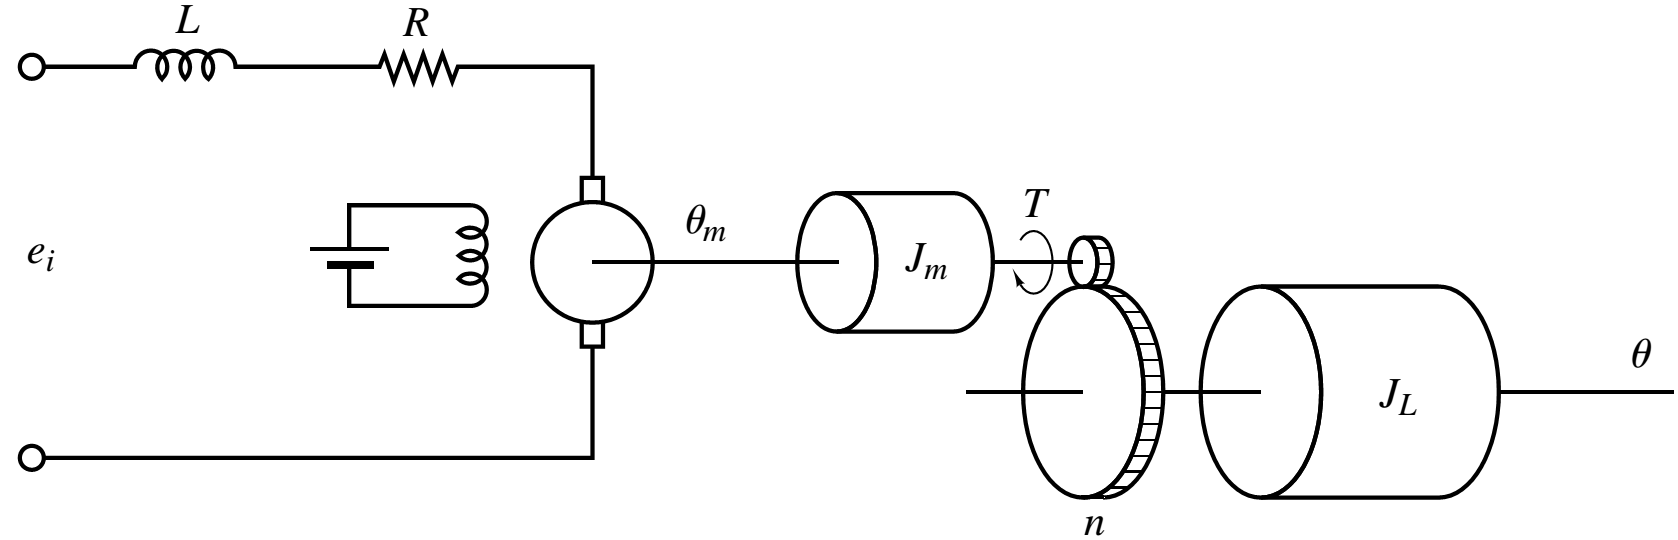
\includegraphics[width=0.7\linewidth]{Images/Q4}
	\caption{Armature-controlled dc servomotor system}
	\label{fig:q4}
\end{figure}
\end{problem}
Let $i_a=$ current in armature circuit, $e_b=K_3\frac{d \theta}{d_t}$ back emf, $K_3=$ back emf constant of the motor and $T= K_2i_a$, where $K_2$ is the motor torque constant. \newline \newline 
%The armature voltage is the output of the amplifier: $e_a=K_1e_v$, where $K_1$ is a gain constant
The equation for torque equilibrium is:
%$J_0\frac{d^2\theta}{dt^2} + b_0\frac{d\theta}{dt} = T = K_2i_a$, where where $J_0$ is the inertia of the combination of the motor, load, and gear train referred to the motor
%shaft and $b_0$ is the viscous-friction coefficient of the combination of the motor, load, and gear train
%referred to the motor shaft. \newline \newline
The armature circuit equation is:
\begin{align}
& L \frac{di_a }{dt}+i_aR+e_b=e_i	\nonumber \\ % formula for armature circuit
& L \frac{di_a }{dt}+i_aR + K_3\frac{d \theta_m}{d_t}=e_i \nonumber \\ % inserted forumla for back emf
& sLI_a(s) + RI_a(s) + sK_3 \Theta_m (s) = E_i(s) 	\label{eq:Q4:1}% laplace transform
\end{align}
The equation for torque equilibrium is:
\begin{align}
& J_0\frac{d^2\theta}{dt^2} + T = T_{motor} = K_2i_a \nonumber \\ % inserted equation 
& T = \frac{\theta}{\theta_m} T_L = n T_L \nonumber \\
& J_L\frac{d^2\theta}{dt^2} = T_L \nonumber \\
& (J_m + n^2J_L)\frac{d^2\theta}{dt^2} = nK_2i_a \nonumber \\ % added parameters from question
& (J_m+n^2J_L)s^2\Theta(s)=nK_2I_a(s) \label{eq:Q4:2} % laplace transform of equation
\end{align}
Eliminating $I_a$ by using equations \ref{eq:Q4:1} and \ref{eq:Q4:2}: \newline
\begin{align*}
& I_a(s)(sL+R)=E_i(s)-sK_3\Theta(s) \\
& I_a(s)= \frac{E_i(s)-sK_3\Theta(s)}{(sL+R)} \\
\end{align*}
\begin{align*}
& (J_m+n^2J_L)s^2\Theta(s)= nK_2 \left(\frac{E_i(s)-sK_3\Theta(s)}{(sL+R)} \right) \\
& \Theta(s)\left((sL+R)\frac{J_m+n^2J_L}{nK_2}\right)s^2 + sK_3 \frac{\Theta(s)}{n}=E_i(s) \\
& \left[\left((sL+R) J_m+n^2J_L \right)s^2 + sK_2K_3 \right]\Theta(s) = nK_2E_i(s) \\
& \boxed{\frac{\Theta(s)}{E_i(s)}= \frac{nK_2}{\left((sL+R) J_m+n^2J_L \right)s^2 + sK_2K_3 } }
\end{align*}

\begin{problem}{5 --- (B)-2-3 --- obtain transfer function} \hfill\newline
	
\begin{figure}[H]
	\centering
	\includegraphics[width=0.7\linewidth]{Circuits/Q5BlockDiagram}
	\caption{Block Diagram for (B)-2--3}
	\label{fig:q5blockdiagram}
\end{figure}
Moving $G_2$ to the left, past a pickoff point results in:
\begin{figure}[H]
	\centering
	\begin{minipage}{.5\textwidth}
		\centering
		\includegraphics[width=1\linewidth]{Circuits/Q5BlockDiagram2}
		\caption{$G_2$ past pick off point}
		\label{fig:prob1_6_2}
	\end{minipage}%
	\begin{minipage}{0.5\textwidth}
		\centering
		\includegraphics[width=1\linewidth]{Circuits/Q5BlockDiagram2-2}
		\caption{Merging $ H_1 \text{and} 1 / G_2$}
		\label{fig:prob1_6_1}
	\end{minipage}
\end{figure}
Combining $\frac{H_1}{G_2}$ and unity, switching the order of the adders before $G_2$ and then using the feedback form results in:
\begin{figure}[H]
	\centering
	\includegraphics[width=1\linewidth]{Circuits/Q5BlockDiagram3}
	\caption{Partially simplifed Block Diagram}
	\label{fig:q5blockdiagram3}
\end{figure}
Collapsing the cascading block diagrams results in and then cascading $G_1$:
\begin{align*}
& G_1\left(\frac{G_2}{1+G_2H_2}\right)\left(1+\frac{H_1}{G_2}\right)G_3=G_1\frac{G_3(G_2+H_1)}{1+G_2H_2} \\
& \text{Then applying the feedback form:} \\ 
& G_1\cfrac{\cfrac{G_3(G_2+H_1)}{1+G_2H_2}}{1+\cfrac{G_3(G_2+H_1)}{1+G_2H_2}H_3}= G_1\cfrac{\cfrac{G_3(G_2+H_1)}{1+G_2H_2}}{\cfrac{1+G_2H_2+H_3G_3(G_2+H_1)}{1+G_2H_2}}= \cfrac{G_1G_3(G_2+H_1)}{1+G_2H_2+H_3G_3(G_2+H_1)}
\end{align*}
\begin{figure}[H]
	\centering
	\includegraphics[width=0.7\linewidth]{Circuits/Q5BlockDiagram4}
	\caption{Feedback Form of (B)-2-3}
	\label{fig:q5blockdiagram4}
\end{figure}
Applying the feedback form a final time results in:
\begin{align*}
& \cfrac{\cfrac{G_1G_3(G_2+H_1)}{1+G_2H_2+H_3G_3(G_2+H_1)}}{1+1\times\cfrac{G_1G_3(G_2+H_1)}{1+G_2H_2+H_3G_3(G_2+H_1)}}= \cfrac{\cfrac{G_1G_3(G_2+H_1)}{1+G_2H_2+H_3G_3(G_2+H_1)}}{\cfrac{1+G_2H_2+H_3G_3(G_2+H_1)+G_1G_3(G_2+H_1)}{1+G_2H_2+H_3G_3(G_2+H_1)}} \\
&= \cfrac{G_1G_3(G_2+H_1)}{1+G_2H_2+H_3G_3(G_2+H_1)+G_1G_3(G_2+H_1)}
\end{align*}
\begin{figure}[H]
	\centering
	\includegraphics[width=0.7\linewidth]{Circuits/Q5BlockDiagram5}
\end{figure}
The transfer function is , $\displaystyle \boxed{\frac{C(s)}{R(s)}= \frac{G_1G_2G_3+G_1G_3H_1}{1+G_2H_2+H_3G_2G_3+H_1H_2G_3+G_1G_2G_3+G_1G_3H_1}}$ 
 \nopagebreak
\end{problem}
\nopagebreak
\begin{problem}[Problem 6 --- (B)-2-7 --- find C(s)/R(s) and C(s)/D(s)] 
To find $ C(s)/R(s)$ set $D(s)=0$ and  for $C(s)/D(s)$ set $R(s)=0$
\begin{figure}[H]
	\centering
	\includegraphics[width=0.7\linewidth]{Circuits/Q6BlockDiagram}
	\label{fig:q6blockdiagram}
\end{figure} 
\textbf{Solving for } $C(s)/R(s)$, set $D(s)=0$, this allows for $G_1$ and $G_2$ to be treated as a cascading system and the new system, $G_1G_2$ is in a feedback form with $H_1$. 
\begin{figure}[H]
	\centering
	\includegraphics[width=0.7\linewidth]{Circuits/Q6BLockDiagram2}
	\caption{Simplified System when $D(s)=0$}
	\label{fig:q6blockdiagram2}
\end{figure}
Using the feedback form again:
\begin{figure}[H]
	\centering
	\includegraphics[width=0.5\linewidth]{Circuits/Q6BLockDiagram3Fin}
	\label{fig:q6blockdiagram3fin}
\end{figure}
\vspace{-0.5cm}
\begin{align*}
& \cfrac{\cfrac{G_cG_3G_1G_2}{1+G_1G_2H_1}}{1+\cfrac{G_cG_3G_1G_2}{1+G_1G_2H_1}} = 
\cfrac{G_cG_3G_1G_2}{1+G_1G_2H_1+G_cG_3G_1G_2}\\
& \boxed{\frac{R(s)}{C(s)} = \frac{G_cG_3G_1G_2}{1+G_1G_2H_1+G_cG_3G_1G_2}}
\end{align*}
\textbf{Solving for } $C(s)/D(s)$, set $R(s)=0$, this allows for $G_c$ and $H_2$ to be treated as a cascading system and moving $G_3$ to the left of a pick off point results in:
\begin{figure}[H]
	\centering
	\includegraphics[width=0.7\linewidth]{Circuits/Q6BLockDiagram4}
	\label{fig:Q6BLockDiagram4}
\end{figure}
Cascading $G_2 + G_3$, $H_2 + G_c$ and $H_1+ 1 / G_3$ and rearranging leads to:
\begin{figure}[H]
	\centering
	\includegraphics[width=0.5\linewidth]{Circuits/Q6BlockDiagram5}
	\label{fig:q6blockdiagram5}
\end{figure}
Using the feedback form:
\begin{figure}[H]
	\centering
	\includegraphics[width=0.5\linewidth]{Circuits/Q6BlockDiagram6fin}
	\label{fig:q6blockdiagram6fin}
\end{figure}
The transfer function, $\displaystyle \boxed{\frac{C(s)}{D(s)}= \cfrac{G_2G_3}{1+G_1G_2G_3G_cH_2+G_1G_2H_1}}$
\end{problem}

\begin{problem}{7 --- B-5-10 --- Matlab plotting} \hfill\newline
The figures \ref{fig:q7step} and \ref{fig:q7rampImpulse} correspond to the plots of the unit-step, unit-ramp and impulse responses plotted in Matlab. The ramp response is the integral of the step response. Thus, multiplying the step response by 1/s and gets the ramp.
\begin{lstlisting}[language = Matlab]
	s = tf('s');
	C = 10;
	R = s^2+2*s+10;
	step(C/R)   % Step response
\end{lstlisting}
\begin{figure}[H]
	\centering
	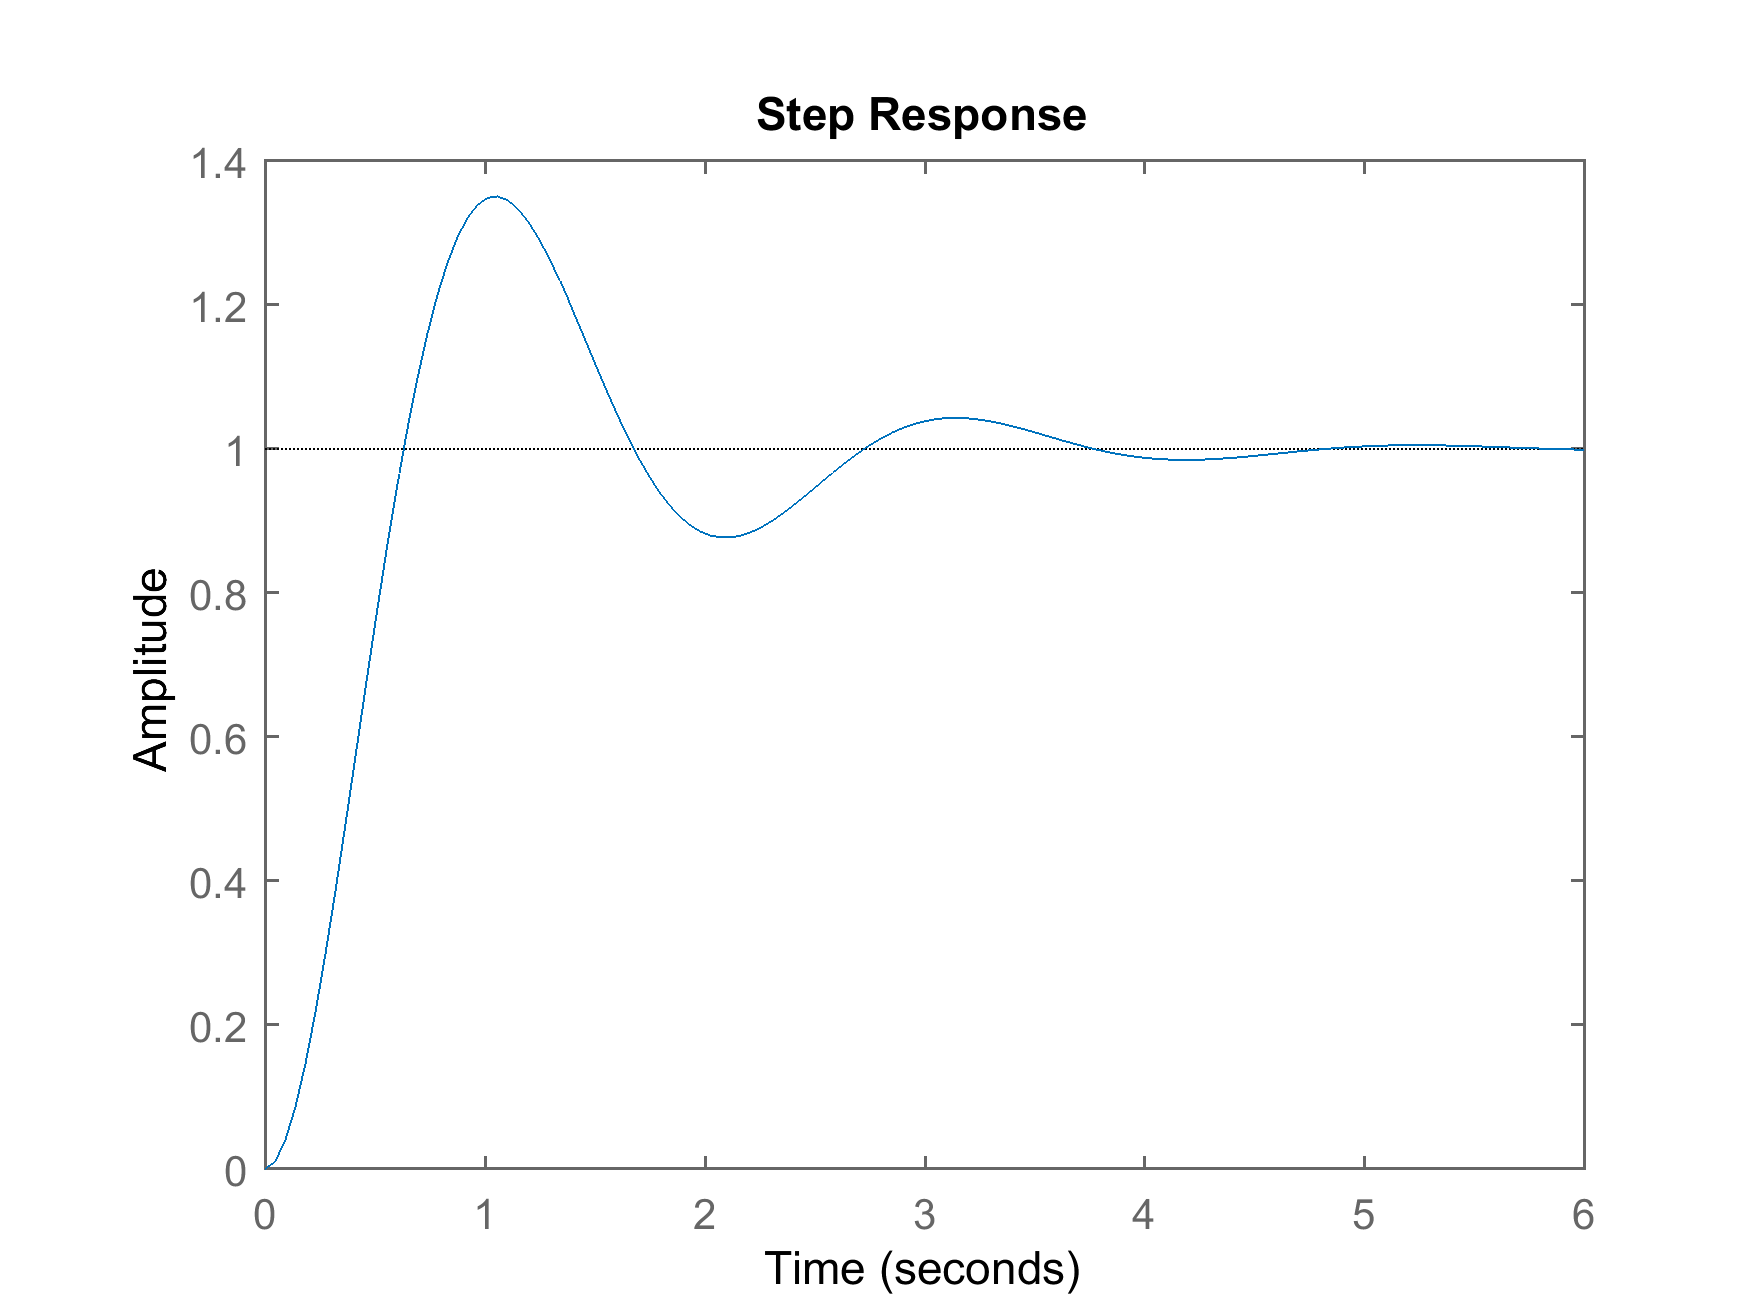
\includegraphics[width=0.5\linewidth]{Images/Q7Step}
	\caption{Step Response for $10 / (s^2+2s+10)$ in Matlab}
	\label{fig:q7step}
\end{figure}
\begin{figure}[H]
	\centering
	\begin{minipage}{.5\textwidth}
		\centering
		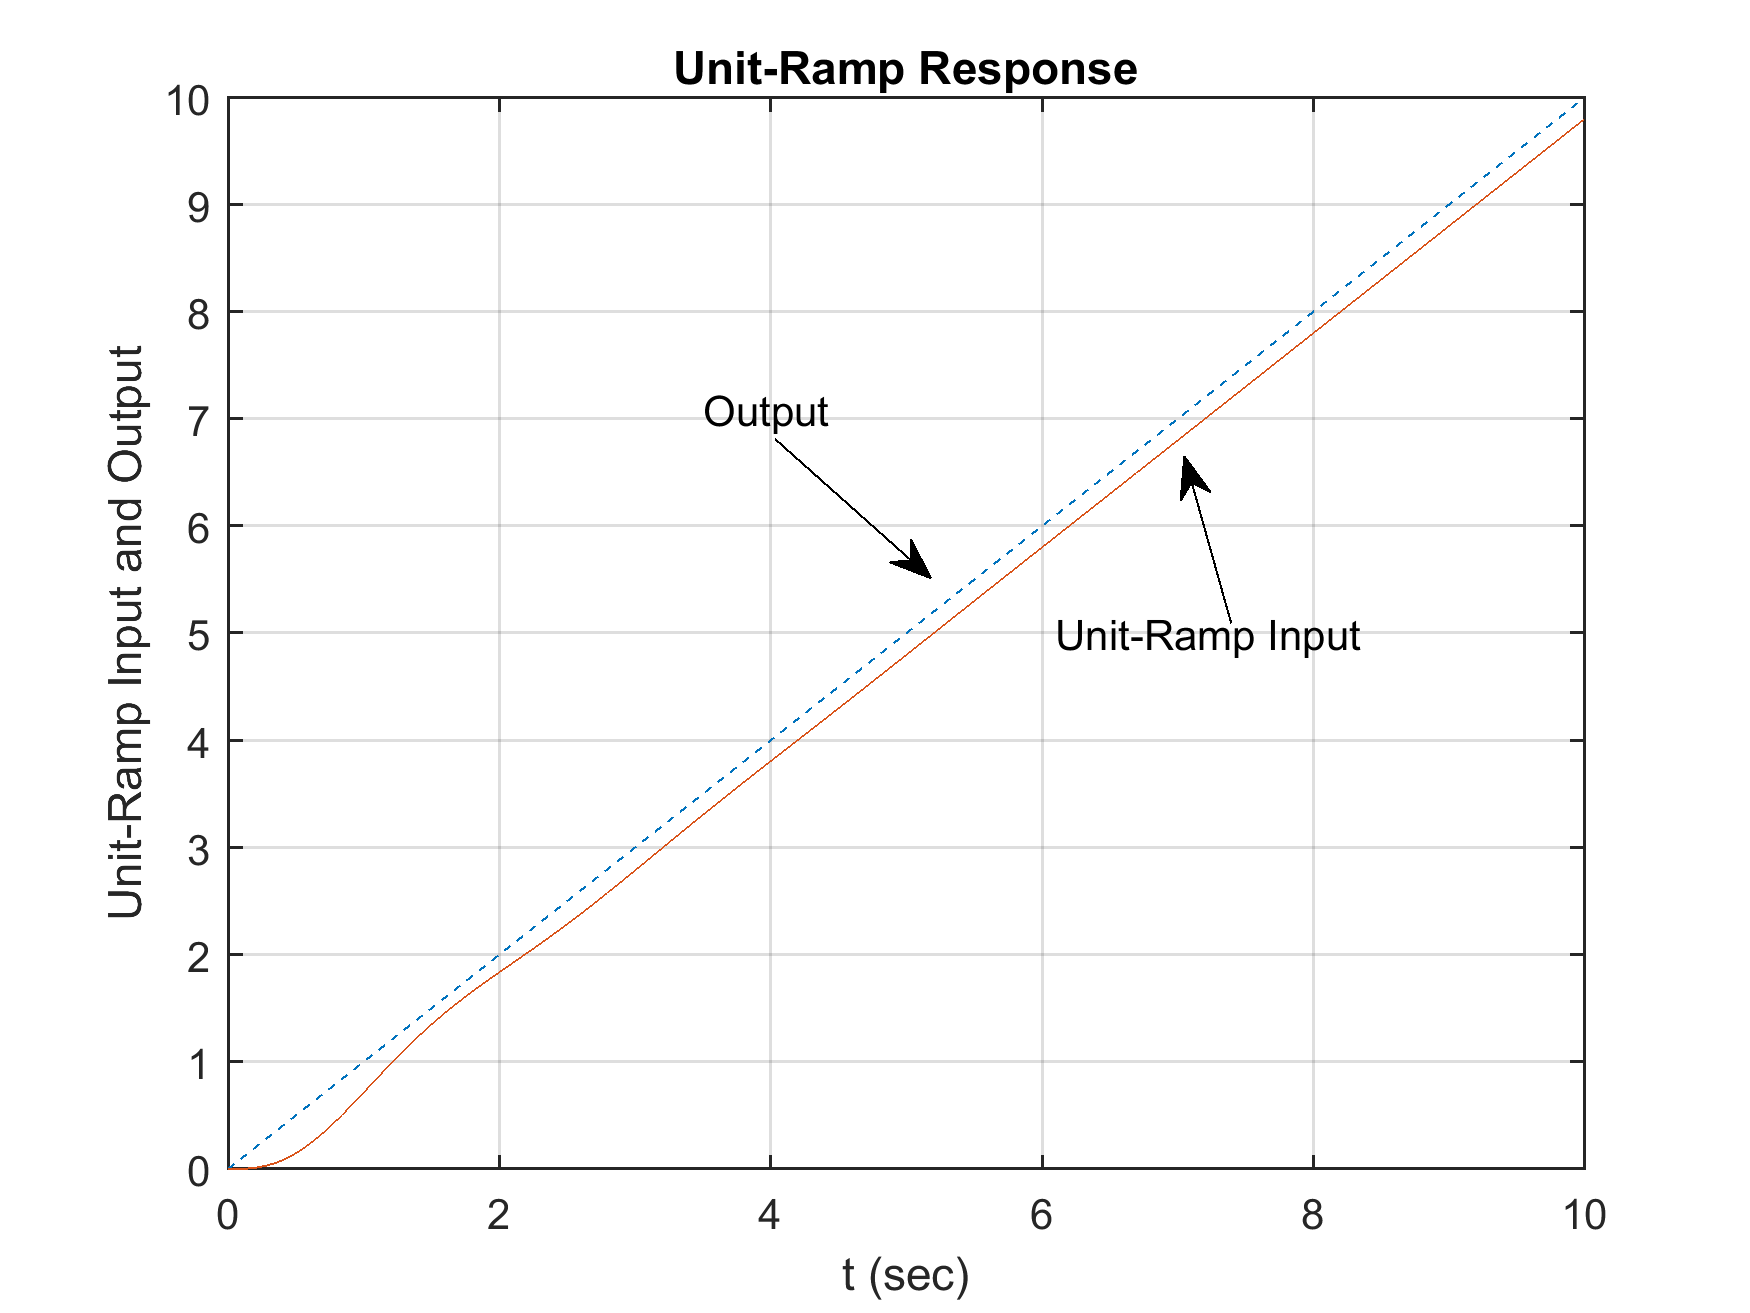
\includegraphics[width=1\linewidth]{Images/Q7RampOgata}
		%	\caption{Ramp Response for $10 / (s^2+2s+10)$ in Matlab}
		\label{fig:q7ramp}
	\end{minipage}%
	\begin{minipage}{0.5\textwidth}
		\centering
		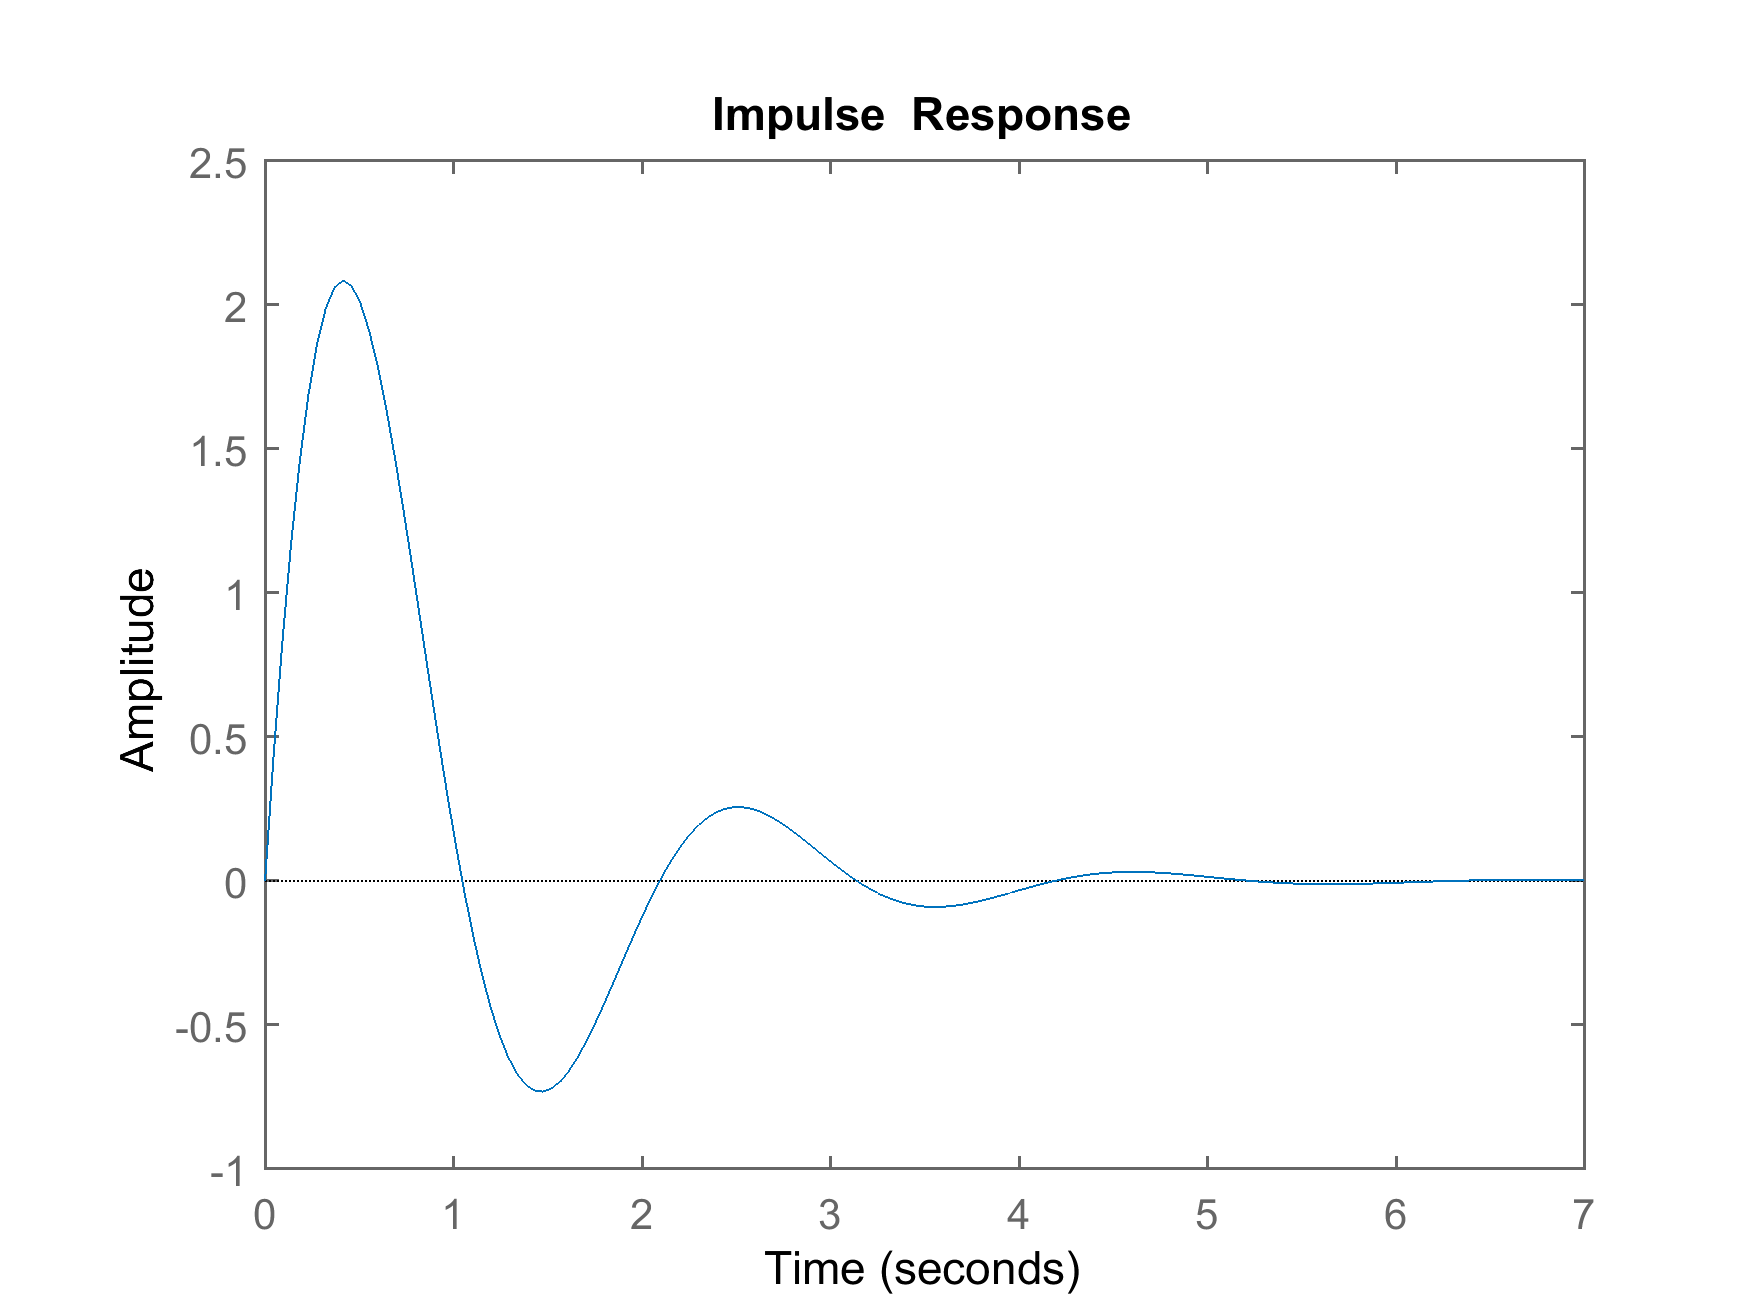
\includegraphics[width=1\linewidth]{Images/Q7Impulse}
		\label{fig:q7impulse}
	\end{minipage}
	\caption{Ramp and Impulse Response for $10 / (s^2+2s+10)$ in Matlab}
	\label{fig:q7rampImpulse}
\end{figure}
\begin{lstlisting}[language = Matlab]
	t = 0:0.02:10;
	num1 = [10];
	den1 = [1 2 10 0];
	y1 = step(num1,den1,t);
	plot(t,t,'--',t,y1)
	v = [0 10 0 10]; axis(v); grid
\end{lstlisting}

\begin{lstlisting}[language = Matlab]
	h = impulseplot(C/R);
	p = getoptions(h);
	p.Title.String =('Impulse Response');
	setoptions(h,p);
\end{lstlisting}

\end{problem}
\begin{problem}{8 --- B-5-12 --- Matlab computations} \hfill\newline
	By plotting and inspecting the step response of the function $\displaystyle=\frac{C(s)}{R(s)}=\frac{36}{s^2+2s+36}$, the values for rise time, peak time, max overshoot and settling time can be computed.
	\begin{figure}[H]
		\centering
		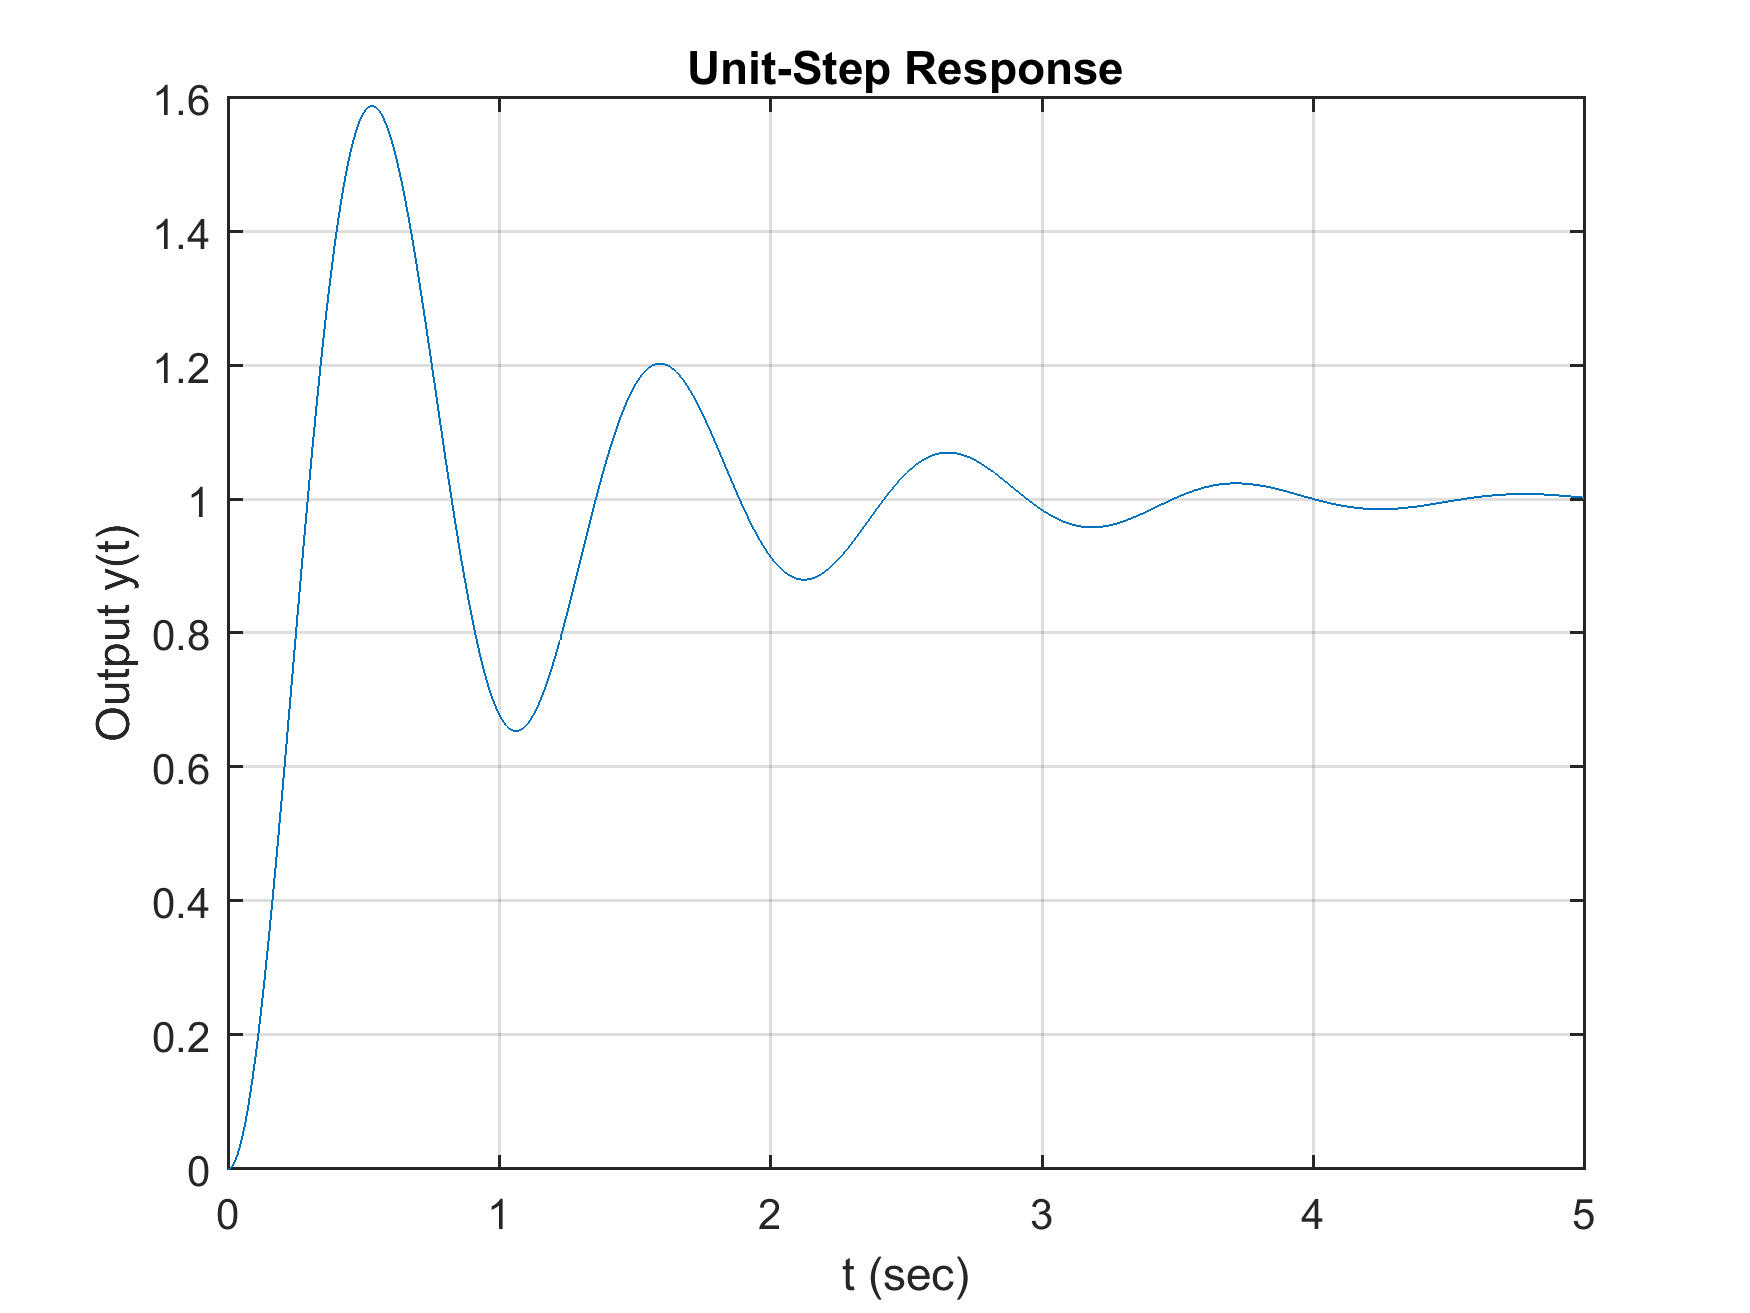
\includegraphics[width=0.5\linewidth]{Images/Q8Step}
		\caption{Step response for Problem B-5-12}
		\label{fig:q8step}
	\end{figure}
\begin{lstlisting}[language = Matlab]
	num = [0 0 36];
	den = [1 2 36];
	t = 0:0.001:5;
	[y,x,t] = step(num,den,t);
	plot(t,y); grid;
	title('Unit-Step Response')
	xlabel('t (sec)')
	ylabel('Output y(t)')
\end{lstlisting}


\begin{lstlisting}[language = Matlab]
	r1 = 1; while y(r1) < 1.0001, r1 = r1+1; end;  
	rise_time = (r1-1)*0.001
	[ymax,tp] = max(y);
	peak_time = (tp-1)*0.001
	max_overshoot = ymax-1	
	s = 5001; while y(s) > 0.98 & y(s) < 1.02; s = s-1; end;
	settling_time = (s-1)*0.001
\end{lstlisting}
\begin{lstlisting}[language = Matlab]
	rise_time =
		0.294000000000000
	peak_time =
		0.531000000000000
	max_overshoot =
		0.588001316697907
	settling_time =
		3.821000000000000
\end{lstlisting}
\end{problem}

\begin{problem}{9 --- B-5-21 --- Routh stability criterion} \hfill\newline
%	B–5–21. Consider the following characteristic equation:
$s^4 + 2s^3 + (4 + K)s^2 + 9s + 25 = 0, a_0=1, a_1=2,a_2=(4+K),a_3=9,a_4=25$ \newline
%	Using the Routh stability criterion, determine the range of
%	K for stability
$ \displaystyle b_1 =\frac{a_1a_2-a_0a_3}{a_1}= \frac{2(4+K)-(4+K)}{2}, b_2=\frac{a_1a_4-a_0a_5}{a_1}=25$  \newline $\displaystyle c_1 =\frac{a_3b_1-a_1b_2}{b_1}=\frac{9(2K-1)/2-2(25)}{(2K-1)/2}=\frac{9K-109/2}{2K-1/2}$
\begin{table}[H]
	\centering
		\renewcommand*{\arraystretch}{2}
\begin{tabular}{l c c c}
		\hline
		$\mathbf{s^4}$&1&(4+K)&25\\\hline
			$\mathbf{s^3}$&2&9&0.00\\\hline
		$\mathbf{s^2}$&$\frac{2K-1}{2}$&25&0.00\\\hline
			$\mathbf{s^1}$&$\frac{9K-109/2}{2K-1/2}$&0.00&0.00\\\hline
			$\mathbf{s^0}$&25.00&0.00&0.00\\\hline
	\end{tabular}
	\caption{Routh-stability calculations}
\end{table}
In order for the system to be stable, the right hand poles, must not exist, therefore $\frac{2K-1}{2} > 0$ and $\frac{9K-109/2}{2K-1/2}>0$, so $K \geq 0.5$ and $\displaystyle \boxed{ K \geq \frac{109}{18} \approx 6.056}$
\end{problem}
\begin{problem}{10 --- B-5-26 --- open loop transfer function-} \hfill\newline
	$\displaystyle \frac{C(s)}{R(s)}=\frac{G(s)}{1+G(s)}=\frac{Ks+b}{s^2+as+b}$
\begin{figure}[H]
	\centering
	\includegraphics[width=0.4\linewidth]{Circuits/Q10BlockDiagram}
	\caption{Closed loop control system transfer function.}
	\label{fig:q10blockdiagram}
\end{figure}
	\begin{align*}
		& G(s)(s^2+as+b)=(1+G(s))(Ks+b) \\
		& G(s)(s^2+as+b-Ks-b)=(Ks+b) \\
		& G(s)=\frac{Ks+b}{s^2+(a-K)s}
	\end{align*}
	The steady-state in the unit-ramp response is:
	\begin{align*}
		& e_{ss}=\frac{1}{K_v}	= \lim\limits_{s \rightarrow 0}\frac{1}{sG(s)}= \lim\limits_{s \rightarrow 0}\frac{s(s+a-K)}{s(Ks+b)}=\frac{a-k}{b}
	\end{align*}
\end{problem}
%\newpage
\newcolumntype{L}{>{\centering\arraybackslash}m{4cm}}
\begin{table}[H]
	\caption*{\Large Time log for ELEC 360 --- Assignment 1}
	\renewcommand*{\arraystretch}{2}
	\begin{tabular}{LLLL}
		\toprule
		\textbf{Week of Sep 10} &  \textbf{Week of Sep 17} &  \textbf{Week of Sep 24} &    \textbf{Week of Oct 1} \\
		\midrule
		2 hours reading pages 13 to 22 of text  &  3 hours spent on deriving transfer functions of example systems &  3 hours spent on preparing for lab &  2 hours doing the prelab and reading textbook \\
		3 hours of internet research on closed loop control system examples &  2 hours towards practising block-diagram reduction techniques &  2 hours towards practising block-diagram reduction techniques &  3 hours reviewing lecture notes and lab report \\
		1 hour of practising Laplace Transform &  2 hours on solving first 4 questions of assignment 1 &  2 hours on solving first 4 questions of assignment 1 &  4 hours solving questions of assignment 1 \\
		\bottomrule
	\end{tabular}
\end{table}
%\begin{figure}
%	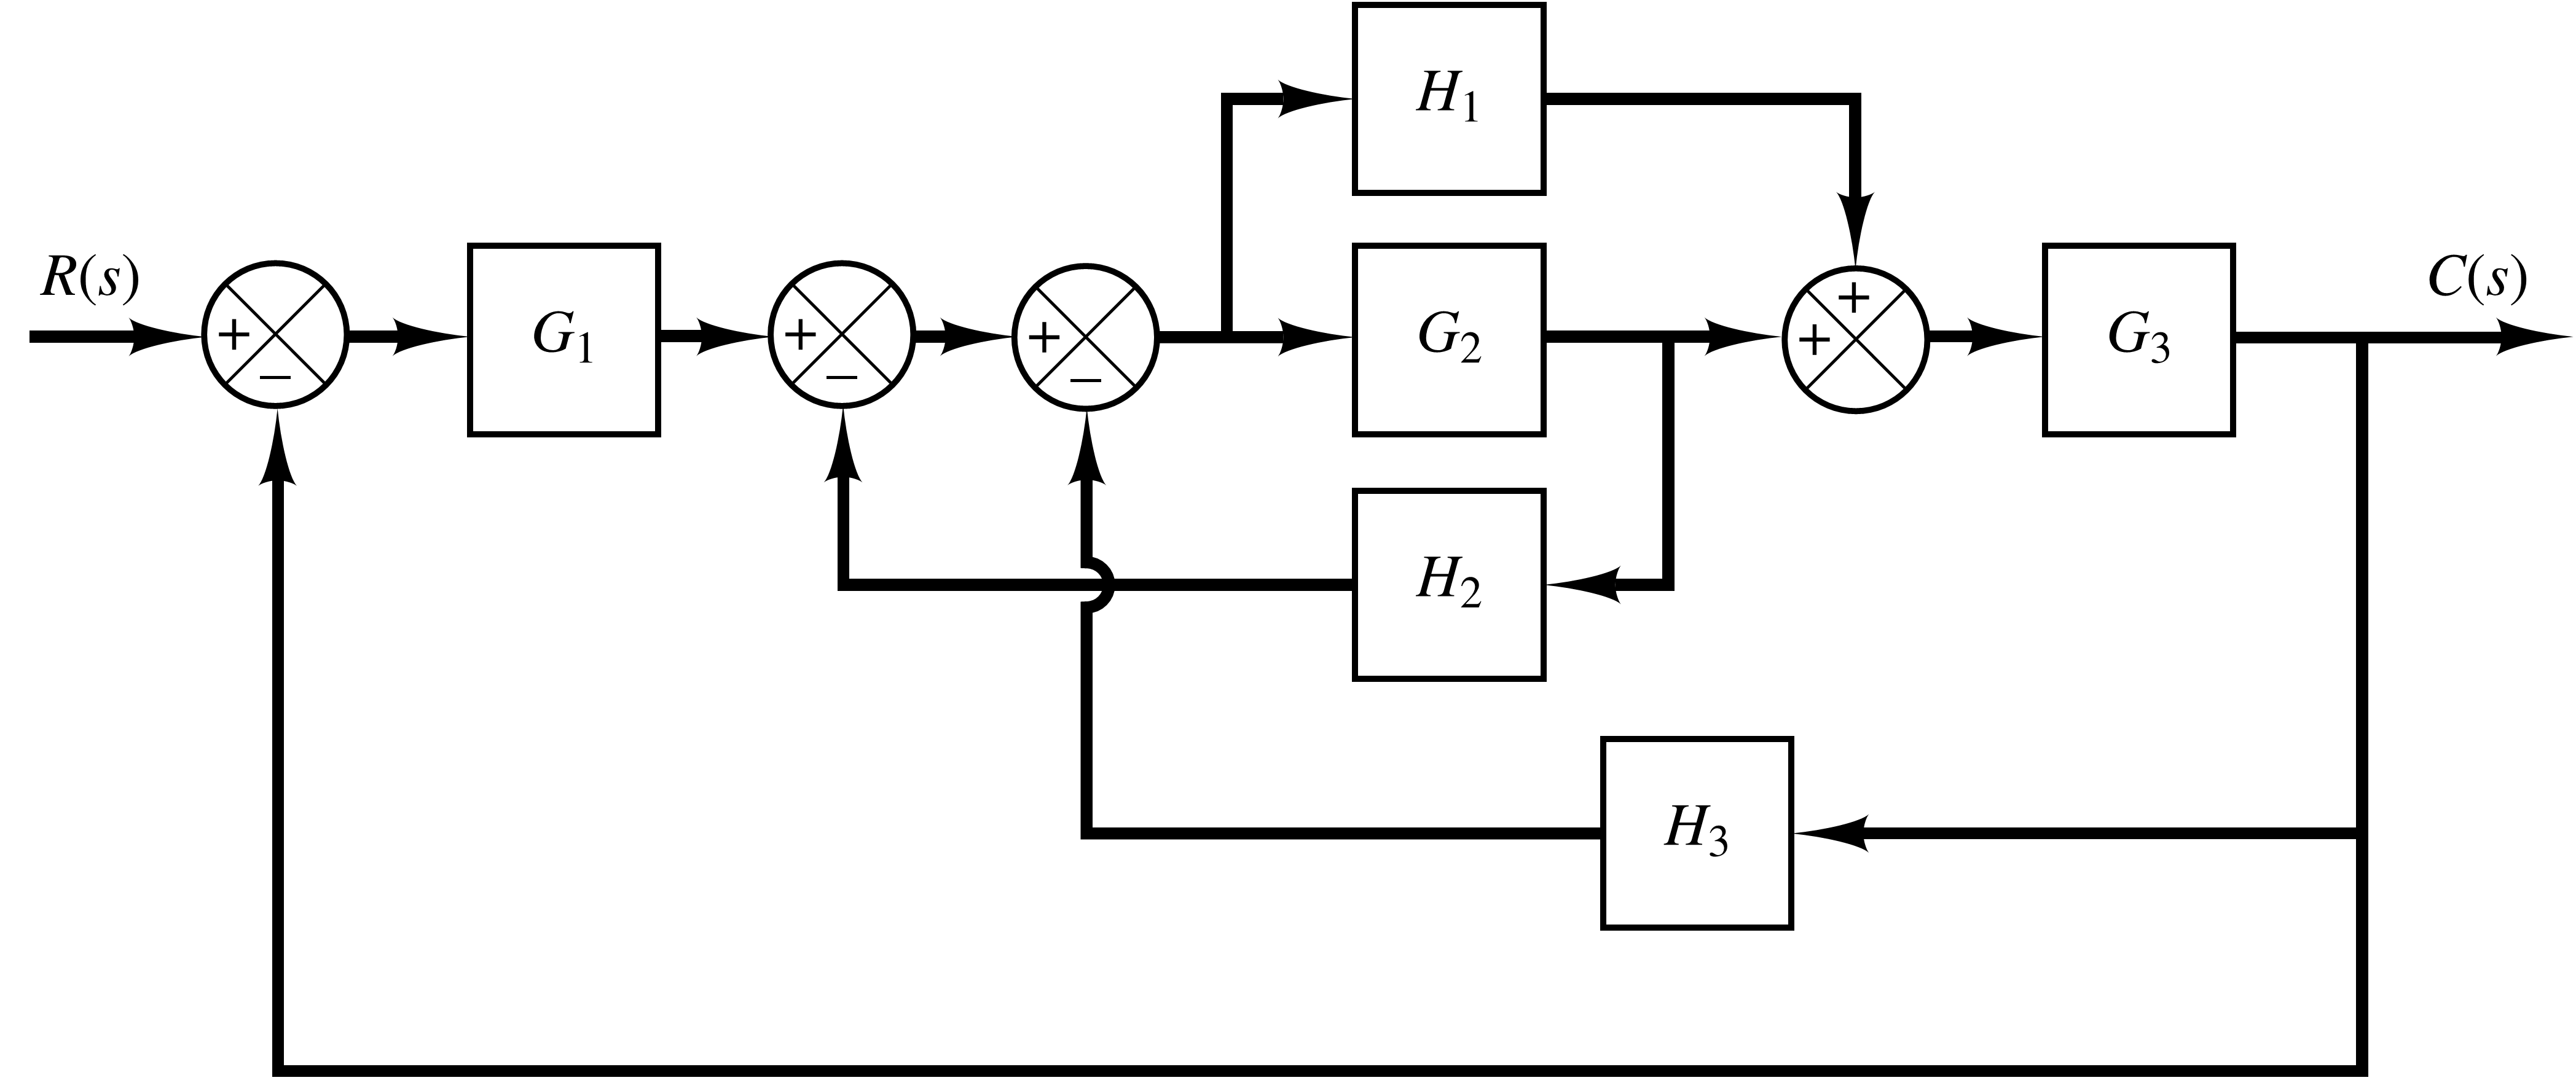
\includegraphics[width=\linewidth]{Images/Q1}
%	\caption{A screenshot of the RTL Schematics produced from the Verilog code.}
%\end{figure}
%	%%%%%%%%%%%%%%%%%%%%%%%%%%%%%%
%	\begin{thebibliography}{1}
%		
%		\bibitem{manual} Lin Cai et al. 2015. Laboratory Manual
%		for CENG460 Communications Networks. University of Victoria, Canada. \\
%		
%		\bibitem{updown} "Computer Hope," [Online]  Available: http://www.computerhope.com/unix/ifup.htm. [Accessed 9 Feburary 2015].
%	\end{thebibliography}
\end{document}

%%%%%%%%%%%%%%%%%%%%%%%%%%%%%%

%%%%%%%%%%%%%%%%
COMMON COMMANDS:
%%%%%%%%%%%%%%%%
% IMAGES
\begin{figure}[H]
	\begin{center}
		\includegraphics[width=0.6\textwidth]{RTL_SCHEM.png}
	\end{center}
	\caption{A screenshot of the RTL Schematics produced from the Verilog code.}
	\label{RTL}
\end{figure}

% SUBFIGURES IMAGES
\begin{figure}[H]
	\centering
	\subfloat[LED4 Period]{\label{fig:Per4}\includegraphics[width=0.4\textwidth]{period_led4.png}} \\                
	\subfloat[LED5 Period]{\label{fig:Per5}\includegraphics[width=0.4\textwidth]{period_led5.png}}
	\subfloat[LED6 Period]{\label{fig:Per6}\includegraphics[width=0.4\textwidth]{period_led6.png}}
	\caption{Period of LED blink rate captured by osciliscope.}
	\label{fig:oscil}
\end{figure}

% INSERT SOURCE CODE
\lstset{language=Verilog, tabsize=3, backgroundcolor=\color{mygrey}, basicstyle=\small, commentstyle=\color{BrickRed}}
\lstinputlisting{MODULE.v}

% TEXT TABLE
\begin{table}
	\begin{center}
		\begin{tabular}{|l|c|c|l|}
			x & x & x & x \\ \hline
			x & x & x & x \\
			x & x & x & x \\ \hline
		\end{tabular}
		\caption{Caption}
		\label{label}
	\end{center}
\end{table}

% MATHMATICAL ENVIRONMENT
$ 8 = 2 \times 4 $

% CENTERED FORMULA
\[  \]

% NUMBERED EQUATION
\begin{equation}

\end{equation}

% ARRAY OF EQUATIONS (The splat supresses the numbering)
\begin{align*}

\end{align*}

% NUMBERED ARRAY OF EQUATIONS
\begin{align}

\end{align}

% ACCENTS
\dot{x} % dot
\ddot{x} % double dot
\bar{x} % bar
\tilde{x} % tilde
\vec{x} % vector
\hat{x} % hat
\acute{x} % acute
\grave{x} % grave
\breve{x} % breve
\check{x} % dot (cowboy hat)

% FONTS
\mathrm{text} % roman
\mathsf{text} % sans serif
\mathtt{text} % Typewriter
\mathbb{text} % Blackboard bold
\mathcal{text} % Caligraphy
\mathfrak{text} % Fraktur

\textbf{text} % bold
\textit{text} % italic
\textsl{text} % slanted
\textsc{text} % small caps
\texttt{text} % typewriter
\underline{text} % underline
\emph{text} % emphasized

\begin{tiny}text\end{tiny} % Tiny
\begin{scriptsize}text\end{scriptsize} % Script Size
\begin{footnotesize}text\end{footnotesize} % Footnote Size
\begin{small}text\end{small} % Small
\begin{normalsize}text\end{normalsize} % Normal Size
\begin{large}text\end{large} % Large
\begin{Large}text\end{Large} % Larger
\begin{LARGE}text\end{LARGE} % Very Large
\begin{huge}text\end{huge}   % Huge
\begin{Huge}text\end{Huge}   % Very Huge


% GENERATE TABLE OF CONTENTS AND/OR TABLE OF FIGURES
% These seem to have some issues with the "revtex4" document class.  To use, change
% the very first line of this document to "article" like this:
% \documentclass[aps,letterpaper,10pt]{article}
\tableofcontents
\listoffigures
\listoftables

% INCLUDE A HYPERLINK OR URL
\url{http://www.derekhildreth.com}
\href{http://www.derekhildreth.com}{Derek Hildreth's Website}

% FOR MORE, REFER TO THE "LINUX CHEAT SHEET.PDF" FILE INCLUDED!

